En nuestra cuarta practica trabajemos con rotaciones en el espacio espectral. A
puntamos con las mismas a poder incorporar conceptos como dimensionalidad y
correlacion entre bandas que nos ayuden a utilizar mejor la informacion
satelital.

Son objetivos de la misma

\begin{itemize}
    \item Aplicar la transformada tasseled cap a una imagen multiespectral e
        interpretar el significado de cada banda.
    \item Poder aplicar la transformada por componentes principales a una imagen
        multiespectral e interpretar el resultado.
    \item Poder aplicar la transformada por componentes principales a un stack
        de bandas multiespectrales de distitnas fechas e interpretar los resultados.
    \item Utilizar la transformada por componentes principales para extraer
        informacion de series temporales de indices.
\end{itemize}

\subsection{Calculo de la transformada tasseled cap para una imagen landsat}

Comencemos calculados la transformada tasseled cap para una imagen landsat. La
misma sera la primer rotacion que utilizaremos en el curso y en ella la
interpretacion es bastante sencilla. Para ello usaremos el paquete
\texttt{RStoolbox}.

\begin{exa}
    Para cualcular la transformada por componentes principales comenzamos
    abriendo la imagen landsat desde el metadado y convirtiendola a reflectancia
    a tope de la atmosfera como vimos en las clases anteriores.
    \begin{lstlisting}
    xml.2016 <- readMeta("raster_data/LC82240782016304/LC82240782016304LGN00.xml")
    ref.2016 <- stackMeta(xml.2016, quantity = "sre")
    scaleF <- getMeta(ref.2016,xml.2016, what = "SCALE_FACTOR")
    ref.2016 <- ref.2016 * scaleF
    ref.2016 <- ref.2016[[-1,]]
    names(ref.2016) <- c("blue","green","red","nir","swir1","swir2")
    \end{lstlisting}
    calculamos analizamos ahora el espacio red-nir y green-nir para la imagen

    \begin{lstlisting}
    B1 <- xyplot(nir~red,data=ref.2016)
    B2 <- xyplot(red~green,data=ref.2016)
    print(B1,split=c(1,1,2,1),more=TRUE)
    print(B2,split=c(2,1,2,1),more=FALSE)
    \end{lstlisting}

    obteniendo como scatterplots

    \begin{figure}[h!]
    \begin{center}
        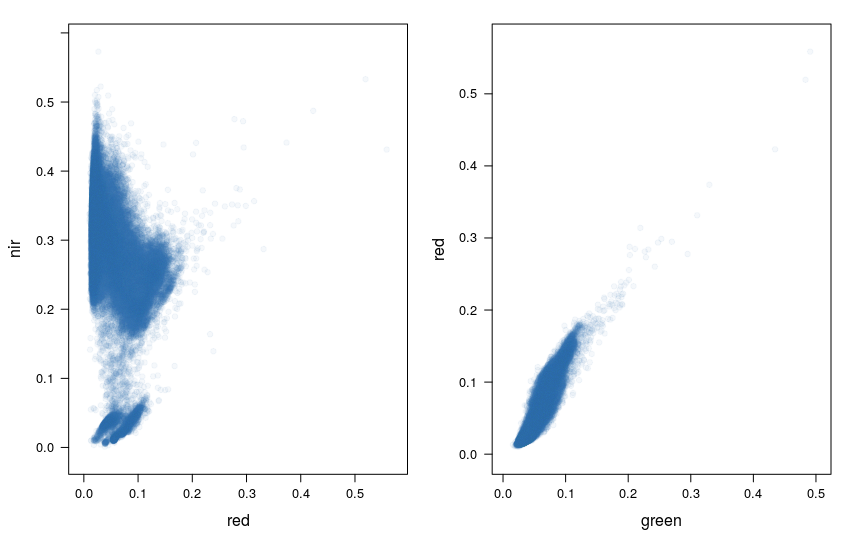
\includegraphics[scale=0.6]{red-nir-green.png}
    \end{center}
    \caption{Scatterplot verde-rojo y nir-red.}
    \label{fig:green-red}
    \end{figure}

    Calculemos ahora la transformada tasseled cap. Para eso usamos la funcion
    \texttt{tasseledCap} del paquete \texttt{RStoolbox}.
    \begin{lstlisting}
    tsc.2016 <- tasseledCap(ref.2016,sat="Landsat8OLI")
    \end{lstlisting}
    Obtenemos una imagen de tres bandas, \emph{brillo}, \emph{verdor} y
    \emph{humedad}.

    podemos graficar cada una de las bandas por separado con el comando

    \begin{lstlisting}
    plot(tsc.2016)
    \end{lstlisting}

    o todas juntas con

    \begin{lstlisting}
    plotRGB(tsc.2016,r=1,g=2,b=3, stretch="lin")
    \end{lstlisting}

    \begin{figure}[h!]
    \begin{center}
        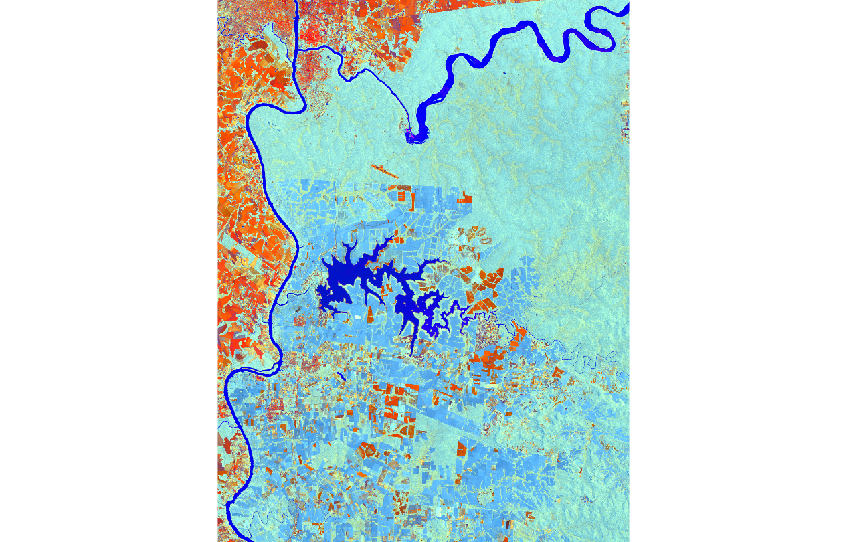
\includegraphics[scale=0.6]{tsc.png}
    \end{center}
    \caption{Imagen de la transformada tasseled cap.}
    \label{fig:tsc}
    \end{figure}
    Vemos en este caso que distintas zonas de la selva presentan distinto color
    en cyan debito al cambio en contenido de humedad, que las zonas sin
    vegetacion se ven en gradientes de rojo igual que las ciudades y las zonas
    cubiertas de agua se ven en azul inenso.
\end{exa}

\begin{act}
    Calcule la transformada tasseled cap para la imagen landsat 7 del año 2000.
\end{act}

\subsection{Calculo de la transformada por componentes principales}

Veamos ahora como calcular la transformada por componentes principales. Para
esto utilizaremos la herramienta \texttt{rasterPCA} del paquete
\texttt{RStoolbox}. Realizaremos ademas un analisis previo sobre las mismas para
ayudar a comprender como funciona dicha transformada.

\begin{exa}
    Comencemos analizando la transformada por componentes principales de la
    imagen de 2016. ¿Que podemos predecir? Miremos primero los
    scatterplots \texttt{pairs(ref.2016)}
    \begin{figure}[h!]
    \begin{center}
        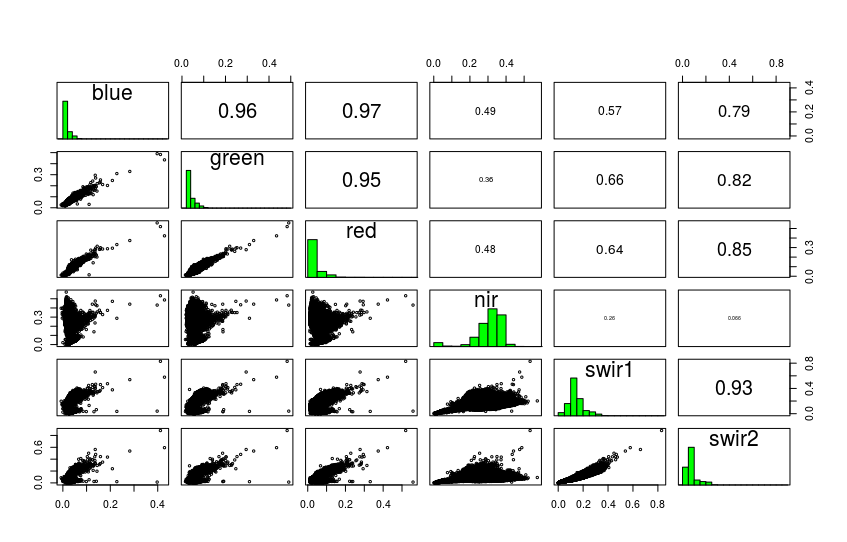
\includegraphics[scale=0.6]{pairs.png}
    \end{center}
    \caption{}
    \label{fig:pairs}
    \end{figure}

    Mirando el resumen de la imagen vemos que hay varias bandas muy
    correlacionadas entre si. Por ejemplo las del visible, mientras que otras lo
    estan poco, por el ejeplo el nir y el swir. Por lo tanto esperamos que no
    todas las bandas sean necesarias para explicar el comportamiento de la
    imagen. Al menos en el nivel de detalle mas baje.

    Apliquemos entonces la transformada por componentes principales y veamos que
    sucede

    \begin{lstlisting}
        pca.2016 <- rasterPCA(ref.2016)
        summary(pca.2016$model)
    \end{lstlisting}

    Veamos el sumario del modelo obtenido,
    \begin{Verbatim}[fontsize=\small]
    Importance of components:
                               Comp.1     Comp.2     Comp.3      Comp.4 ...
    Standard deviation     0.08079854 0.07808556 0.01242745 0.006488765 ...
    Proportion of Variance 0.50850204 0.47492732 0.01202957 0.003279516 ...
    Cumulative Proportion  0.50850204 0.98342936 0.99545892 0.998738441 ...
    \end{Verbatim}

    Al analizar las varianzas, vemos que las 3 primeras explican mas que el
    99.5\% de la variabilidad de la imagen. Es decir, que de las 6 bandas de
    landsat 8, en esta imagen, 3 nos alcanzan para explicar casi todo el
    comportamiento. Analisemos la primera, usamos el comando
    \texttt{loadings(pca.2016\$model)} para ver como son las componentes.

    \begin{Verbatim}[fontsize=\small]
    oadings:
          Comp.1  ...
    blue
    green
    red   -0.128  ...
    nir   -0.575  ...
    swir1 -0.663  ...
    swir2 -0.451  ...
    \end{Verbatim}

    la primer componente pesa, segun la banda pero siempre con el mismo signo, a
    todas las demas componentes. Podemos interpretarla por lo tanto como un
    brillo y esperar que sea mas alta cuando miramos  zonas de la imagen que
    tengan mas reflectancia en promedio

    Si mostramos las tres primeras componentes en combinacion RGB vemos que
    distintos tipos de coberturas se distinguen de distinta manera,

    \begin{lstlisting}
    plotRGB(pca.2016$map,r=1,g=2,b=3, stretch="lin")
    \end{lstlisting}

    Vale la pena aclarar en este caso que debemos referenciar el mapa dentro del
    objeto pca y no directamente el objeto para graficarlo.
\end{exa}

\begin{act}
    Analice la segunda componente de la transformada por componentes principales
    para la imagen Landsat 8.
\end{act}

\begin{act}
    Calcule y analice la transformada por PCA de la imagen Landsat 7 del año
    2000.
\end{act}

\subsection{Algunas ideas sobre series temporales}

Empecemos esta seccion con una actividad para que realicen

\begin{act}
    Aplique la transformada por componentes principales al stack de bandas del
    año 2000 y 2016.
\end{act}

Veamos que pasa al trabajar con series temporales de indices.

\begin{exa}
    Otra aplicacion de la transformada por componentes principales por
    componentes principales es el analisis de series temporales.
    \begin{lstlisting}
    ndvi.list <- list.files("raster_data/MOD13Q1/NDVI/", pattern = "*.tif$",
                             full.names = TRUE)
    ndvi.stack <- stack(ndvi.list)
    \end{lstlisting}
    una vez abierta la imagen la convertimos a valores entre -1 y 1 e
    interpolamos los valores faltantes.
    \begin{lstlisting}
    ndvi.stack <- ndvi.stack/1e4
    ndvi.stack <- approxNA(ndvi.stack)
    writeRaster(ndvi.stack,"ndvi-series.tif")
    \end{lstlisting}
    Una vez llenados los espacios donde no habia datos podemos abrir la imagen
    en qgis y realizar consultas de pixel en distintas zonas de la misma.

    Utilizando la herramienta de identificar objetos espaciales podemos
    consultar como es el comportamiento de la serie temporal para cada pixel.
    \begin{figure}[h!]
    \begin{center}
        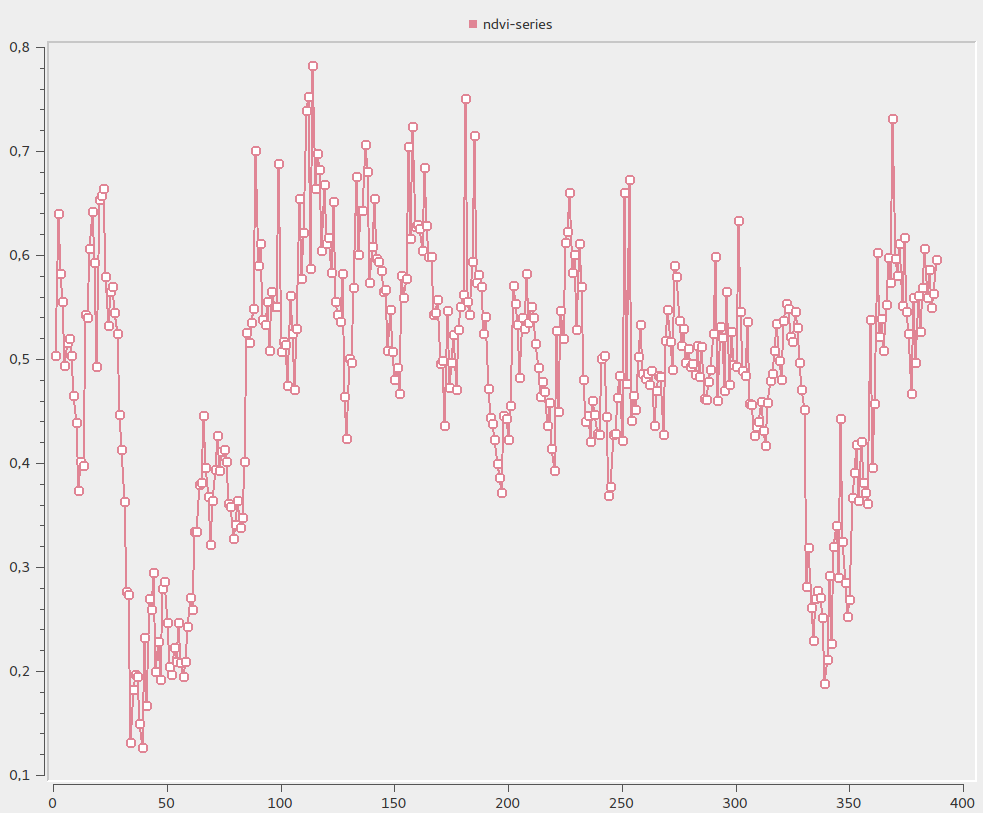
\includegraphics[scale=0.3]{series.png}
    \end{center}
    \caption{}
    \label{fig:series}
    \end{figure}
    vemos que distintas zonas tienen distintos comportamiento intra e
    interanual.

    Podemos analizar el promedio y el desvio standar para cada pixel de la
    imagen
    \begin{lstlisting}
    ndvi.mean <- mean(ndvi.stack)
    plot(ndvi.mean)
    ndvi.sd <- calc(ndvi.stack, fun=sd)
    plot(ndvi.sd)
    \end{lstlisting}
\end{exa}

\begin{act}
    Grafique las primeras 4 componentes por de la transformada por componentes
    princiales de la imagen del stack de NDVI\@. Que zonas puede identificar en la
    primera? que zonas se distinguen en la segunda? que comportamiento encuentra
    en la tercera y cuarta.
\end{act}

\begin{act}
    Grafique en el scatter-plot la imagen completa y marque en el mismo zonas
    con vegetacion, agua y suelo sin cobertura vegetal. Vea como cambian estas
    zonas frente a las transformadas por componentes principales y tasseled cap.
\end{act}
